\chapter{Swarm coordination - area flooding}\label{chapter:flooding}
Area flooding is a technique used to fill an enclosed area with agents such that they are distributed as `effectively' as possible throughout an area. An optimum distribution of agents is not necessarily an even distribution. The distribution of the agents is governed by the field effects and the interaction of agents with obstacles (\textit{interaction vectors}). 

Filling an area can be applied to tasks that require an unknown environment to be analysed or surveyed. Consider a disaster area following a landslide or a building collapsing following an earthquake; the movement in the land and buildings will produce spaces that are unmapped. The unmapped areas may require investigation to locate people, resources or to create some form of sensor network to analyse the conditions within the area such as creating a heat map or to identify the location toxic gases. 

This thesis demonstrates two swarm expanding techniques using field effects to perform area filling for the purposes described above.

The concept of using a swarm to provide coverage over unknown areas is a current area of research. Alvissalim et al. (2012) discuss the application of commercially available drones to provide a communication infrastructure across an unknown disaster areas~\cite{AZHMJJM:12}. Scheutz and Bauer (2006) use both cohesion and repulsion as a mechanism to create coverage of an area that requires protection in an adversarial environment~\cite{SB:06}. The technique used by Scheutz and Bauer (2006) is similar to the principle of \textit{goal-based swarms} as discussed in chapter~\ref{chapter:coordination}. In their paper they do not use cohesion to ensure the swarm remains a cohesive unit, rather they have all the agents using a \textit{destination vector} to cause agents to converge on a target and the repulsion vector prevents collisions. The cohesive effect is not required due to all agents having a common goal with no requirement for the agents to remain in close proximity during the terrain traversal. Ramaithitima et al. in 2015 and 2016, working as part of Vijay Kumar's research group at the University of Pennsylvania, use the idea of filling an area through a deployment strategy that requires the swarm to identify the placement of agents in a given space. The agents are then `shuffled' into an identified position. The technique applied in 2015~\cite{RWBK:15} is based upon coverage path planning and involves adding agents when required and does not require a global positioning reference. In their 2016 paper~\cite{RWBK:16} they use Voronoi graphs to achieve the same effect. Yang et al. (2015)~\cite{YDH:15} also use Voronoi graphs to achieve their swarm coverage goal. The use of Voronoi graphs requires inter-agent communications. Schroeder and M. Kumar (2016) use the bio-inspired swarming technique of creating chemical trails (pheromones) combined with a foraging approach which they refer to as a `food foraging' technique~\cite{SK:16}.

The techniques used in this thesis are similar to Schroeder and M. Kumar in that the agents do not require a global positioning system and differ from Alvissalim et al., Scheutz and Bauer, and Ramaithitima et al. in that the space filling is achieved with a fixed sized swarm. 

The expansion fill is implemented using two techniques. The main principle behind both techniques is to increase the repulsion field effect of the agents over time to increase the area coverage of the agents. The expansion fill can use both the cohesion and repulsion field effects in a similar manner to a static swarm in free space. This technique ensures all the agents remain in close proximity and as far as possible the agents form a single entity. Alternatively the expansion fill can be implemented using only a repulsion field effect. Cohesion can be eliminated in an enclosed space as the agents have a limited range of movement (bounded by a perimeter). When agents move to a repulsion boundary, either an area perimeter or an obstacle, they are repelled. As the space is finite the repulsion `pushes' the agents back into the swarm countering the expansion that is induced by the \textit{interaction vectors}. If the repulsion field effect creates a swarm that reaches all the boundaries the repulsion imposes a compression effect as the \textit{interaction-vector} `pushes' the agents into the boundaries. 

\section{Field effect modification with cohesion and repulsion}
The concept behind the field effect expansion is to increase both the repulsion and cohesion fields over a period of time. This increase in the field effects makes the agents increase the distance between each other expanding the swarm as a whole. The expansion increases until, due to boundary compression, the swarm is unable to expand further. In an extreme case the expansion will result in a set of field effects that create a mesh based swarm structure rather than the desired hexagonal structure that the field effects should create. Identifying either the change in modality or the inability to expand, which can be identified by the \textit{inter-agent vector magnitude} increase or a reduction in the inter-agent distance stability indicates area saturation has occured.

To test this hypothesis a swarm is modelled in the simulator. The model consists of an obstacle-based enclosed space and a swarm consisting of 60 agents. The experiments parameters for the simulation are shown in~\autoref{tab:FillParameters}

\begin{table}[H]
\begin{center}
\begin{tabular}{| p{2.5cm} | p{2.0cm} | p{6.0cm} |}
\hline
\bf Parameter & \bf Value  & \bf Description \\ \hline
$k_c$         & 5          & weight adjuster for cohesion bias\\ \hline
$k_r$         & 60         & weight adjuster for repulsion bias\\ \hline
Sample rate   & 100ms      & proximity sensor rate\\ \hline
Speed         & 20 units/s & agent speed\\ \hline
\end{tabular}\caption{Swarm parameters} \label{tab:FillParameters}
\end{center}
\end{table}

The field effects are incremented in turn, neighbour range followed by repulsion range. After each repulsion field change the swarm is allowed to redistribute itself and stabilise. \autoref{tab:emerge:BaselineConcaveReduction} shows the field effect settings that are used for the simulation. The field effect are selected so as to ensure the swarm parameters have the potential to create a hexagonal swarm. 

\begin{table}[H]
\begin{center}
\begin{tabular}{| p{2cm} | p{0.6cm} | p{0.6cm} | p{0.6cm} | p{0.6cm} | p{0.6cm} | p{0.6cm} | p{0.6cm} | p{1cm} |}
\hline
\bf Weight \bf component & \bf 1 & \bf 2 & \bf 3 & \bf 4 & \bf 5 & \bf 6 & \bf 7 & \\ \hline
Repulsion Boundary & 50 & -  & 60 & -  & 70 & -  & 80 & units\\  \hline
Neighbour Distance & 60 & 70 & -  & 80 & -  & 90 & -  & units\\  \hline
\end{tabular}\caption{field effect expansion sequence} \label{tab:FillSequence}
\end{center}
\end{table}

\autoref{methods:ExpansionFill} shows the stages that the swarm progresses through during the simulation. \autoref{emerge:Expand1} shows the initial deployment of the 60 agents within the enclosed environment. \autoref{emerge:Expand6} shows the stage at which the experiment terminates due to area saturation.

\begin{figure}[H]
\centering
\subfigure[Stage 1]{
	 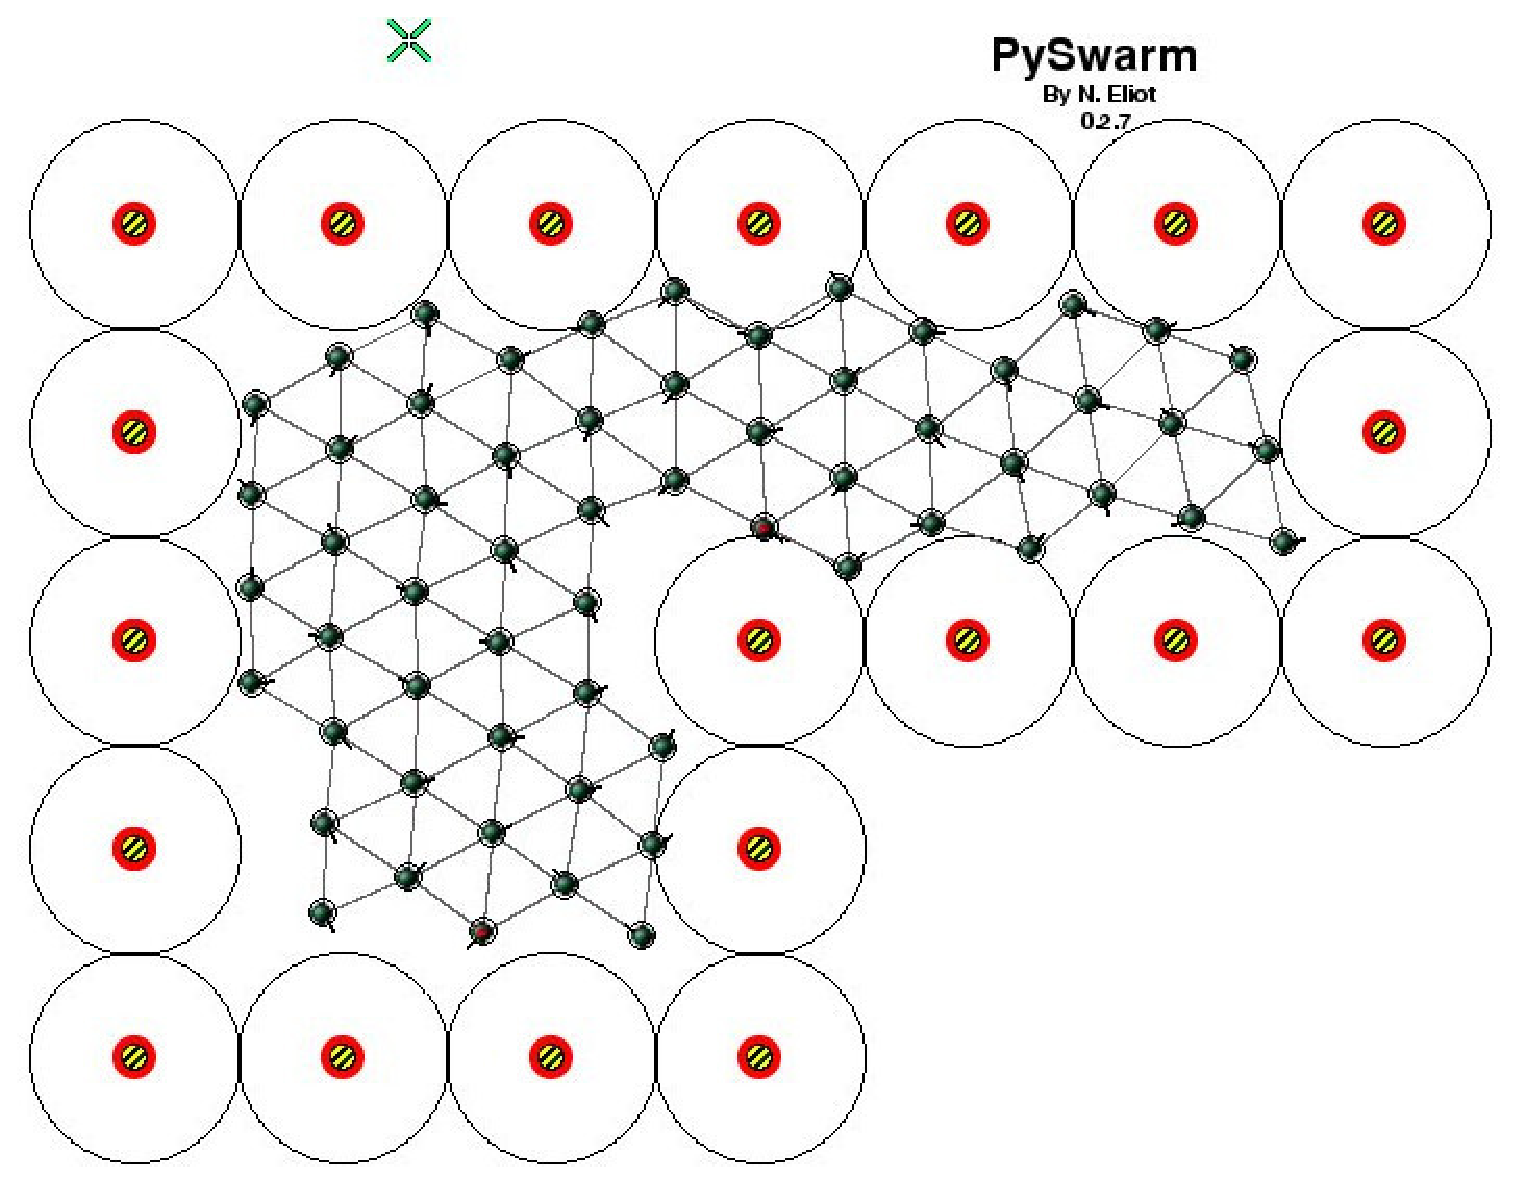
\includegraphics[width=6cm]{CHAPTER-8/figures/EXPAND1}
	 \label{emerge:Expand1}
}
\subfigure[Stage 2]{
	 \includegraphics[width=6cm]{CHAPTER-8/figures/EXPAND2}
	 \label{emerge:Expand2}
}
\subfigure[Stage 3]{
	 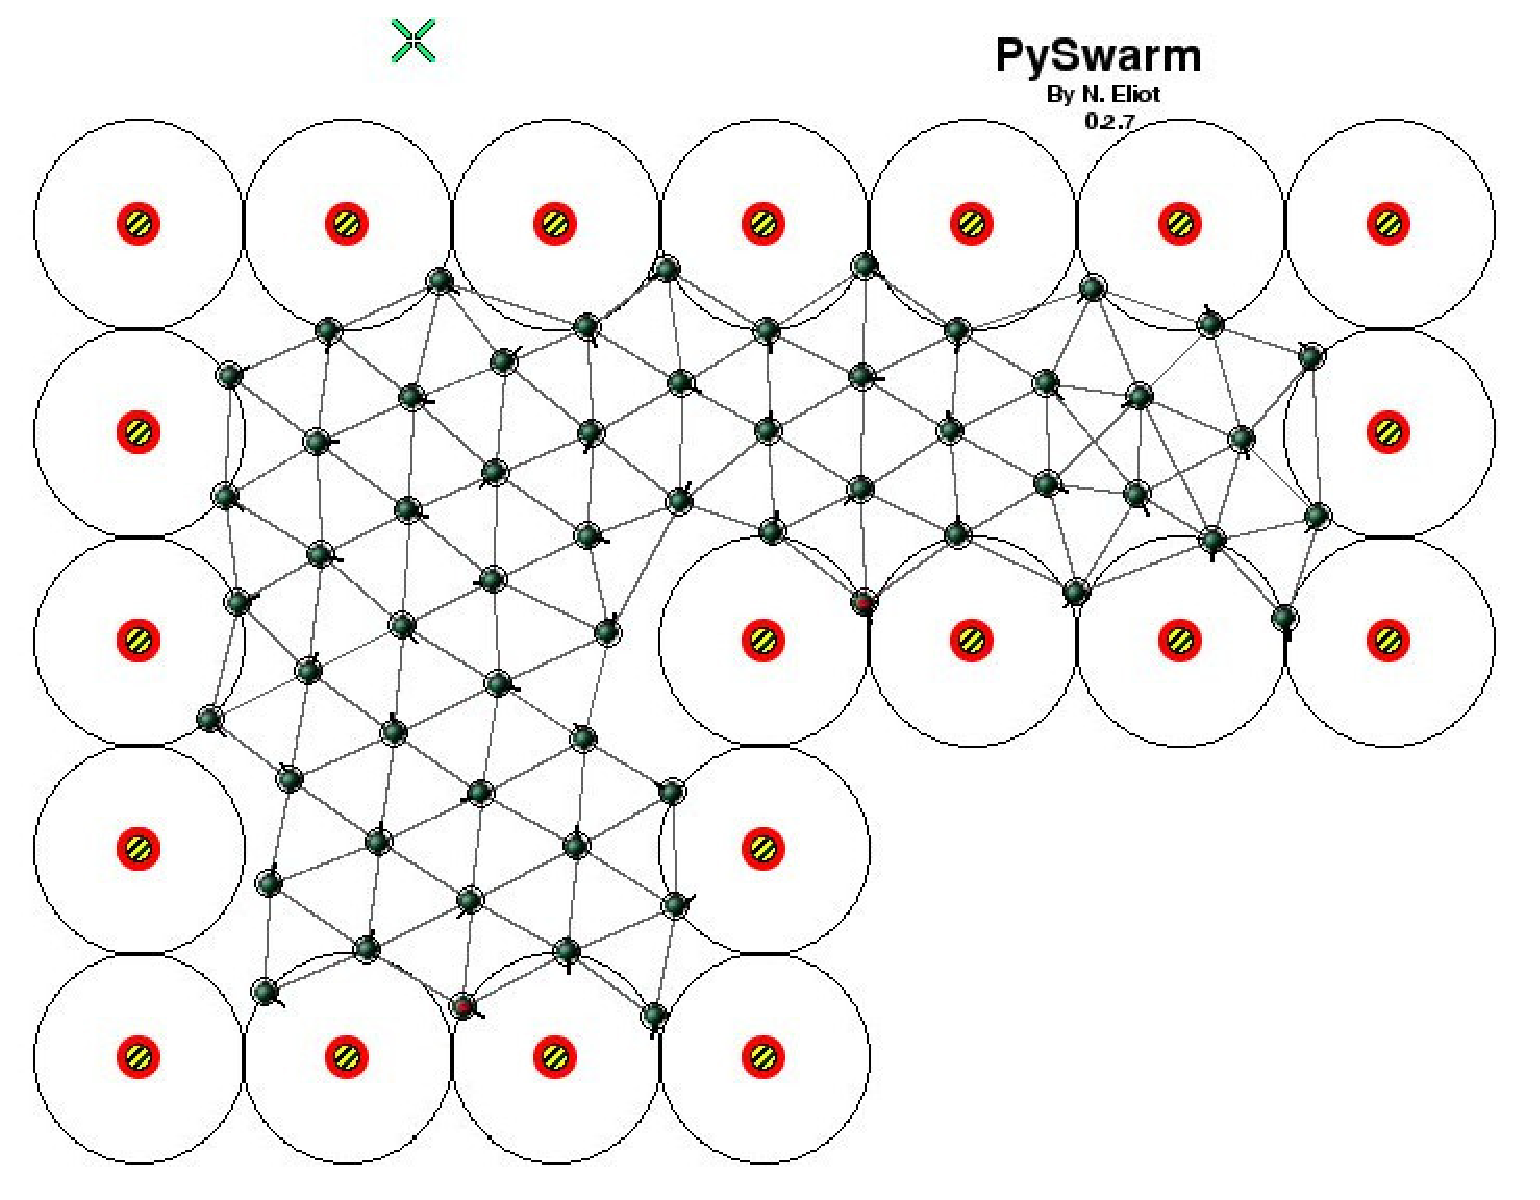
\includegraphics[width=6cm]{CHAPTER-8/figures/EXPAND3}
	 \label{emerge:Expand3}
}
\subfigure[Stage 4]{
	 \includegraphics[width=6cm]{CHAPTER-8/figures/EXPAND4}
	 \label{emerge:Expand4}
}
\subfigure[Stage 5]{
	 \includegraphics[width=6cm]{CHAPTER-8/figures/EXPAND5}
	 \label{emerge:Expand5}
}
\subfigure[Stage 6]{
	 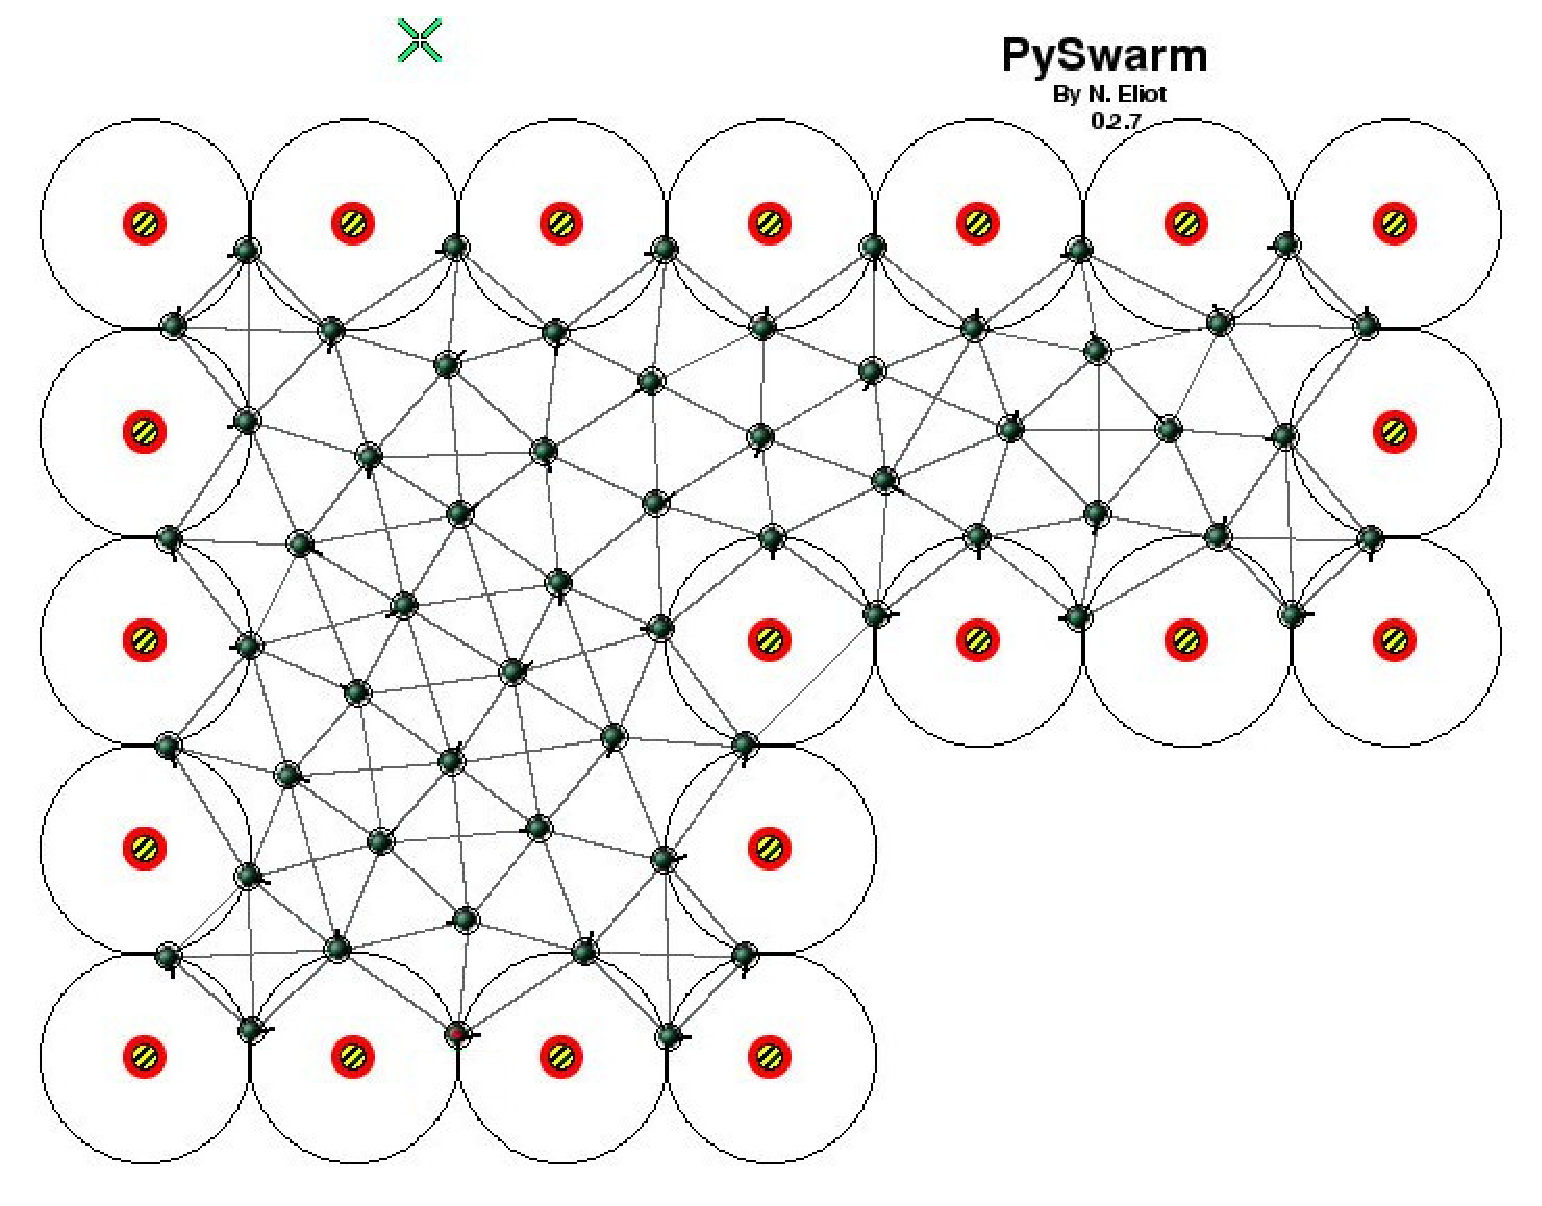
\includegraphics[width=6cm]{CHAPTER-8/figures/EXPAND6}
	 \label{emerge:Expand6}
}
\caption{Space filling via field effect expansion}
\label{methods:ExpansionFill}
\end{figure}

After the initial deployment the system is allowed to settle~(\autoref{emerge:Expand2}) following the settling period the parameters are increased and the swarm settles again. \autoref{emerge:Expand3}~shows how the change in parameters can cause the system to become unstable, the top right section of the swarm has became multi-modal yet there is still a section of the swarm that has not expanded to the boundary perimeter. As the swarm stabilises this compressed section of the swarm `pushes' through the swarm and the swarm increases in volume filling more of the space~(\autoref{emerge:Expand4}). This process continues until changes in the parameters are unable to increase the distribution of the agents and the distances remain almost constant. Increasing the field effects further causes the swarm to become multi-modal as shown in~\ref{emerge:Expand5} and~\ref{emerge:Expand6}.

These effects can be identified through a combination of the \textit{inter-agent magnitude metric} and the distance metric.

\subsection{Magnitude analysis}
\autoref{emerge:FIELDFILL-MAG} shows the resultant magnitude for the swarm for the entire simulation. Between 100 seconds and 105 seconds there is a significant change in the magnitude where the value becomes negative. This indicates there is a compression effect on the swarm and it is unable to expand the inter-agent distances.

\begin{figure}[H]
\begin{center}
\includegraphics[width=12cm]{CHAPTER-8/figures/FIELDFILL-MAG}
\end{center}
\caption{Magnitude metric 0-120 seconds\label{emerge:FIELDFILL-MAG}}
\end{figure}

\autoref{emerge:FIELDFILL-MAG-1} shows the initial deployment status of the swarm and the first repulsion increase at 25 seconds. When the repulsion field is increased, the average \textit{inter-agent magnitude} falls and the variation increases. The agents redistribute themselves which takes until approximately 65 seconds and a new baseline is established for the field effects.

\begin{figure}[H]
\begin{center}
\includegraphics[width=12cm]{CHAPTER-8/figures/FIELDFILL-MAG-1}
\end{center}
\caption{Magnitude metric 0-60 seconds\label{emerge:FIELDFILL-MAG-1}}
\end{figure}

The next increment at 65 seconds creates a similar reaction to the magnitude and variance and the swarm settles to another baseline, however, the new baseline has a variance which drops the resultant magnitude to below zero. This indicates that some of the swarm is experiencing a compression effect which will result in the swarm body moving towards an uncompressed area. At 85 seconds the next repulsion increase is made and the reaction of the swarm metrics indicates something has changed in how the swarm is reacting. The average \textit{inter-agent magnitude} rises and the variance increases. This change is the effect of an increase in the modality of the swarm which indicates that the swarm is fully distributed within the environment as the neighbour field effect is detecting additional neighbour agents. The final increment at 108 seconds creates an even greater increase in the variance, this is caused by a further increase in the modal distribution of the agents and the swarm is being compressed by the boundary of the space.

\begin{figure}[H]
\begin{center}
\includegraphics[width=12cm]{CHAPTER-8/figures/FIELDFILL-MAG-2}
\end{center}
\caption{Magnitude metric 60-120 seconds\label{emerge:FIELDFILL-MAG-2}}
\end{figure}

\subsection{Distance analysis}
\autoref{emerge:FIELDFILL-DIST}~shows the distance metric for the simulation. The initial deployment is shown at 0 seconds followed by incremental changes in the distances and variance of the distances as each increment is made in the field effects. The simulation terminates after 12 seconds.

\begin{figure}[H]
\begin{center}
\includegraphics[width=12cm]{CHAPTER-8/figures/FIELDFILL-DIST}
\end{center}
\caption{Distance metric 0-120 seconds\label{emerge:FIELDFILL-DIST}}
\end{figure}

\autoref{emerge:FIELDFILL-DIST-1} shows the initial expansion increasing the field distance causing the agents to `spread' throughout the space. Each increment having a settling period as the swarm expands.

\begin{figure}[H]
\begin{center}
\includegraphics[width=12cm]{CHAPTER-8/figures/FIELDFILL-DIST-1}
\end{center}
\caption{Distance metric 0-60 seconds\label{emerge:FIELDFILL-DIST-1}}
\end{figure}

\autoref{emerge:FIELDFILL-DIST-2}~shows the simulation from 60-120 seconds. Between 60 and 85 seconds an increment is made in the field effects and the swarm expands. At 85 seconds there is further increment, however the effect on the distribution is different. The distribution of the agents has changed due to the modality of the swarm. The average distance has increased and there is an increase in the variance. This would indicate that the swam has fully expanded and is unable to expand further. The final increment at 105 seconds can be seen to further impact on the modality indicating the area is saturated.

\begin{figure}[H]
\begin{center}
\includegraphics[width=12cm]{CHAPTER-8/figures/FIELDFILL-DIST-2}
\end{center}
\caption{Distance metric 60-120 seconds\label{emerge:FIELDFILL-DIST-2}}
\end{figure}

\subsection{Combined magnitude and distance analysis}
Combining the results of the distance and \textit{inter-agent magnitude} metrics provides a more indepth view of the effects changing the field effects has upon the swarms structure.

There is a significant change in the \textit{inter-agent magnitude} when the field effects are incremented to 70 units for repulsion and 80 units for neighbour distance~(Figures \ref{emerge:FIELDFILL-MAG-3} and \ref{emerge:FIELDFILL-MAG-3b}). There is no significant change in the inter-agent distances~(Figures \ref{emerge:FIELDFILL-DIST-3} and \ref{emerge:FIELDFILL-DIST-3b}). Until this point the average \textit{inter-agent magnitude} is positive which indicates an aggregate cohesion in the swarm. After the increment there is an aggregate repulsion in the swarm indicating the swarm is being compressed and the repulsion field effect vector magnitude is greater than the cohesion field effect vector magnitude. A positive cohesion does not indicate the space is not filled only that the swarm still shows a tendency to remain a cohesive entity.

\begin{figure}[H]
\begin{center}
\includegraphics[width=12cm]{CHAPTER-8/figures/FIELDFILL-DIST-3}
\end{center}
\caption{Distance metric 80-110 seconds\label{emerge:FIELDFILL-DIST-3}}
\end{figure}

\begin{figure}[H]
\begin{center}
\includegraphics[width=12cm]{CHAPTER-8/figures/FIELDFILL-MAG-3}
\end{center}
\caption{Magnitude metric 80-110 seconds\label{emerge:FIELDFILL-MAG-3}}
\end{figure}

\begin{figure}[H]
\begin{center}
\includegraphics[width=12cm]{CHAPTER-8/figures/FIELDFILL-DIST-3b}
\end{center}
\caption{Distance metric 100-120 seconds\label{emerge:FIELDFILL-DIST-3b}}
\end{figure}

\begin{figure}[H]
\begin{center}
\includegraphics[width=12cm]{CHAPTER-8/figures/FIELDFILL-MAG-3b}
\end{center}
\caption{Magnitude metric 100-120 seconds\label{emerge:FIELDFILL-MAG-3b}}
\end{figure}

\section{Field effect modification with repulsion only}
The previous mechanism for area filling used both repulsion and cohesion to ensure the swarm remains, as far as is possible, a single entity. When using repulsion only it is accepted that the agents are in a restricted area and not being cohesive is not and issue as the field effects can be expanded until the agents interact with each other and the boundary. A similar approach was used by Scheutz and Bauer in 2006~\cite{SB:06}. The repulsion field effect in this thesis is used with a fixed sized swarm and the repulsion field is increase over time. The simulation for this experiment uses 52 agents in the same confined space as the previous experiment. The parameters are shown below: 

\begin{table}[H]
\begin{center}
\begin{tabular}{| p{2.5cm} | p{2.0cm} | p{6.0cm} |}
\hline
\bf Parameter & \bf Value  & \bf Description \\ \hline
$k_c$         & 0          & weight adjuster for cohesion vector\\ \hline
$k_r$         & 15         & weight adjuster for repulsion vector\\ \hline
Sample rate   & 100 ms      & proximity sensor rate\\ \hline
Speed         & 20 units/s & agent speed\\ \hline
\end{tabular}\caption{Swarm parameters repulsion only} \label{tab:FillParameters}
\end{center}
\end{table}

\begin{table}[H]
\begin{center}
\begin{tabular}{| p{2cm} | p{0.6cm} | p{0.6cm} | p{0.6cm} | p{0.6cm} | p{0.6cm} | p{0.6cm} | p{1cm} |}
\hline
\bf Weight \bf component & \bf 1 & \bf 2 & \bf 3 & \bf 4 & \bf 5 & \bf 6 & \\ \hline
Repulsion Boundary & 50 & 51 & 52 & 53 & 54 & 55 & units\\  \hline
Neighbour Distance & 70 & 70 & 70 & 70 & 70 & 70 & units\\  \hline
\end{tabular}\caption{field effect expansion sequence} \label{tab:emerge:BaselineConcaveReduction}
\end{center}
\end{table}

The theory behind this type of flood filling is as follows; Cohesion and repulsion acting against each other causes jitter, removing the cohesion allows the swarm to expand to its maximum volume with all agents distributed so they no longer interact at which point jitter will cease. The boundary created by the enclosed space will effect the expanding swarm by repelling the agents back into the swarm preventing expansion therefore the swarm movement will propogate to fill vacant areas. Jitter will initially be seen as the swarm equalises and it will decrease to zero when the swarm is fully expanded. There will be a point in the swarms expansion when the agents will not be able to extend to a zero repulsion point and there will be a permanent interaction between the perimeter and agents. This condition is the exit point for the repulsion flood fill.

\autoref{emerge:SwarmFloodRepel} shows the stages that a field-repulsion-area-fill propagates through. The initial deployment is shown in~\autoref{emerge:Repel52-1}. When the simulation starts the swarm immediately expands~(\autoref{emerge:Repel52-2}) and all the agents stabilise to a position where their movement stops. The field effect is increased and the swarm distribution movement commences. This cycle continues until the swarm is unable to resolve to a neutral expansion point.

\begin{figure}[H]
\centering
\subfigure[Stage 1]{
	 \includegraphics[width=6cm]{CHAPTER-8/figures/REPEL52-1}
	 \label{emerge:Repel52-1}
}
\subfigure[Stage 2]{
	 \includegraphics[width=6cm]{CHAPTER-8/figures/REPEL52-2}
	 \label{emerge:Repel52-2}
}
\subfigure[Stage 3]{
	 \includegraphics[width=6cm]{CHAPTER-8/figures/REPEL52-3}
	 \label{emerge:Repel52-3}
}
\subfigure[Stage 4]{
	 \includegraphics[width=6cm]{CHAPTER-8/figures/REPEL52-4}
	 \label{emerge:Repel52-4}
}
\subfigure[Stage 5]{
	 \includegraphics[width=6cm]{CHAPTER-8/figures/REPEL52-5}
	 \label{emerge:Repel52-5}
}
\subfigure[Stage 6]{
	 \includegraphics[width=6cm]{CHAPTER-8/figures/REPEL52-6}
	 \label{emerge:Repel52-6}
}
\subfigure[Stage 7]{
	 \includegraphics[width=6cm]{CHAPTER-8/figures/REPEL52-7}
	 \label{emerge:Repel52-7}
}
\subfigure[Stage 8]{
	 \includegraphics[width=6cm]{CHAPTER-8/figures/REPEL52-8}
	 \label{emerge:Repel52-8}
}
\caption{Space filling via repulsion}
\label{emerge:SwarmFloodRepel}
\end{figure}

\subsection{\textit{Inter-agent magnitude} analysis}
\autoref{emerge:REPELFILL5055-MAG} shows the \textit{inter-agent vector magnitude} produced between the agents. The initial deployment of the swarm shows a large negative value due to the swarm being in a highly compressed state. This causes the swarm to expand rapidly. Following the initial expansion the agents enter a phase of very close adjustment as their positions move towards a maximum expansion point. Eventually the agents are distributed to their maximum positions with the \textit{inter-agent vector magnitude} stabilises to zero with no variation. At this stage the swarm has stopped moving. This effect cannot be detected by using the distance metric which will simply show a distribution distance with a fixed variance. Having a fixed variance does not indicate the agents have stopped moving as agents could be moving in sympathy to each other creating a net change of zero.

\begin{figure}[H]
\begin{center}
\includegraphics[width=12cm]{CHAPTER-8/figures/REPELFILL5055-MAG}
\end{center}
\caption{Magnitude metric 0-450 seconds\label{emerge:REPELFILL5055-MAG}}
\end{figure}

\autoref{emerge:REPELFILL5055-MAG-1-2} shows the initial settling period of the swarm in greater detail between 0 and 65 seconds. The graph shows that the settling period lasts for approximately 55 seconds following the initial expansion of the swarm from 0 to 10 seconds. The initial deployment of swarm has a highly negative \textit{interaction vector magnitude} causing rapid expansion. From 10 second until approx 62 seconds the agents \textit{inter-agent vectors} cause the agents to spread within the space. When the agents reach the limits of the repulsion field effect they stop moving. The \textit{inter-agent vector magnitude} stabilises to zero and all the agents stop moving.

\begin{figure}[H]
\begin{center}
\includegraphics[width=12cm]{CHAPTER-8/figures/REPELFILL5055-MAG-1-2}
\end{center}
\caption{Magnitude metric 0-65 seconds\label{emerge:REPELFILL5055-MAG-1-2}}
\end{figure}

\autoref{emerge:REPELFILL5055-MAG-2-3} shows a detailed view of the magnitude for the swarm at the first repulsion field increment at approximately 73.5 seconds. The repulsion field effect is incremented by 1 unit. The field effect change is sufficient to allow agents to be within the neighbour field effect range. The agents are already distributed from the initial expansion so there is a `trickling' movement that occurs as the agents increase the area of the swarm within the space. The area containment is not causing any disturbance to the swarm at this stage so the swarm settles to zero (84.5 seconds). As with the initial expansion all the agents are distributed such that they are on or beyond the limits of the repulsion field effect and the swarm stops moving. This process of incrementing the field effect and the swarm stablising continues until the field effect causes the swarm to expand to a point that it fills the area and the agents are unable to move sufficiently to stop interacting.

\begin{figure}[H]
\begin{center}
\includegraphics[width=12cm]{CHAPTER-8/figures/REPELFILL5055-MAG-2-3}
\end{center}
\caption{Magnitude metric 70-85 seconds\label{emerge:REPELFILL5055-MAG-2-3}}
\end{figure}

\autoref{emerge:REPELFILL5055-MAG-8} shows the final part of the simulation where the swarm's resultant magnitude is unable to stabilise completely. The graph shows the increment at approximately 230 seconds creating swarm movement which slowly increasing towards zero as the swarm expands however the \textit{inter-agent vector magnitude} is not able to reach zero. The swarm's agents are bound by the space and cannot distribute themselves to a point where the field effect overlap is overcome. The \textit{inter-agent vector magnitude} average remains below 0 indicating there is a `pressure' that cannot be overcome and the agents are in continuous movement. At this stage it is possible for all the agents to obtain a state of equilibrium and for the average magnitude to stablise but owing to their containment the average magnitude would not be able to rise to zero. The swarm has therefore expanded to fill the space.

\begin{figure}[H]
\begin{center}
\includegraphics[width=12cm]{CHAPTER-8/figures/REPELFILL5055-MAG-8}
\end{center}
\caption{Magnitude metric 235-315 seconds\label{emerge:REPELFILL5055-MAG-8}}
\end{figure}

\subsection{Distance analysis}
\autoref{emerge:REPELFILL5055-DIST} shows the distance metric for the same simulation as above. The initial deployment shows the agents are quite close together but immediately expand, the variance reduces as the agents become more evenly distributed. 

\begin{figure}[H]
\begin{center}
\includegraphics[width=12cm]{CHAPTER-8/figures/REPELFILL5055-DIST}
\end{center}
\caption{Distance metric 0-450 seconds\label{emerge:REPELFILL5055-DIST}}
\end{figure}

\autoref{emerge:REPELFILL5055-DIST-1} shows the period when the swarm has initially expanded to a point that the distances appear to stabilise. The stable state is shown as a constant average distance with a constant variance. It cannot be assumed that the agents have stopped moving at this point in the simulation. Agents could change positions such that the average variance is unaffected although this is unlikely. Over this same period the magnitude is zero as shown in~\autoref{emerge:REPELFILL5055-MAG}. These two facts therefore allow the swarms state to be fully realised. The agents are distributed unevenly and are static.

\begin{figure}[H]
\begin{center}
\includegraphics[width=12cm]{CHAPTER-8/figures/REPELFILL5055-DIST-1}
\end{center}
\caption{Distance metric 60-75 seconds\label{emerge:REPELFILL5055-DIST-1}}
\end{figure}

\autoref{emerge:REPELFILL5055-DIST-1-2} shows the effect of the first increment of the repulsion field effect increment (50-51 units). The swarm agents move to equalise the \textit{inter-agent vectors} by increasing the distance between the agents. The average distance changes very little due to the irregular distribution of the agents (there is no cohesion to help balance the distribution). The variance in the distance has reduced as the agents are more evenly distributed. At this stage the agents are not filling the space (\textit{inter-agent vector magnitude} has resolved to 0)~(\autoref{emerge:REPELFILL5055-MAG-2-3}). The two metrics together indicate that the swarm's agent distribution is more even but the swarm is not filling the space.

\begin{figure}[H]
\begin{center}
\includegraphics[width=12cm]{CHAPTER-8/figures/REPELFILL5055-DIST-1-2}
\end{center}
\caption{Distance metric 70-85 seconds\label{emerge:REPELFILL5055-DIST-1-2}}
\end{figure}

\autoref{emerge:REPELFILL5055-DIST-2-3} shows that at each increment the inter-agent average distances varies but the variance decreases as the swarm stabilises and the distribution improves. This improvement in distribution is the agents `spreading' more evenly as the swarm expands within the area. However after the last field effect increase at 230 seconds the swarm is no longer able to stabilise to a static state. 

\begin{figure}[H]
\begin{center}
\includegraphics[width=12cm]{CHAPTER-8/figures/REPELFILL5055-DIST-2-3}
\end{center}
\caption{Distance metric 180-280 seconds\label{emerge:REPELFILL5055-DIST-2-3}}
\end{figure}

\autoref{emerge:REPELFILL5055-DIST-8} shows the effect of the final increment. The swarm expands but is unable to stabilise the system. The average distances fluctuate as the agents move to balance the \textit{inter-agent vectors} but the distances are unable to increase any further. The inter-agent distances are effected by the positioning of some of the agents preventing a regular shape to be formed this causes the distance variance to increase and the swarms structure starts to oscillate. These characteristics indicate that the area may be fully filled. The magnitude at this point is below zero~\autoref{emerge:REPELFILL5055-MAG-8} which indicates expansion of the swarm is posible but not occuring. The conclusion therefore is that the swarm is fully expanded. The magnitude indicates a tendency for the swarm to expand but the distances are not increasing in line with the magnitude increase. 

\begin{figure}[H]
\begin{center}
\includegraphics[width=12cm]{CHAPTER-8/figures/REPELFILL5055-DIST-8}
\end{center}
\caption{Distance metric 235-315 seconds\label{emerge:REPELFILL5055-DIST-8}}
\end{figure}

\section{Conclusion}
Both of the flood fill techniques work successfully in filling the space. The use of the distance metric is limited in showing the full state state of a swarm due there being no indication of a static state. The \textit{inter-agent vector} metric provides an indication of the ability of the swarm to expand. Using the two metrics together allows the level of the flood filling of a space to be identified. A large distribution in distances indicates possible spaces in the distribution of the agents and ensuring the average \textit{inter-agent vector magnitude} becomes negative ensures the swarm will resolve anomalies in the distribution.

The difference in the approaches of using cohesion combined with repulsion and repulsion only provide two very different characteristics for determining the exit condition for the flood fill. The combination of repulsion and cohesion fields together result in a swarm that moves not only to fill the space but also to accommodate inter-agent relationships as a result the swarm is unable to obtain a static state. Using repulsion only provides clear indications when the space is not filling a space and allows `gaps' to occur in the swarms structure as the cohesion is not present even when agents are within visible `range'.